% !TeX root = ../main.tex

\chapter{概要设计}
本章是在需求分析的基础上对整个仿真平台我所完成的模块设计及设计空间探索
模块的设计进行简要的阐述。在此章节中,我们可以清晰的了解到硬件模型生成模块
(Processor模块和Memory模块)、GeneralFifo模块设计及设计空间探索的流程,
为具体实现打好基础。

\section{系统整体结构}
整个系统整体结构主要包括两个部分:仿真平台部分,包括硬件平台
构建、调度器模块、任务图解析及仿真部分;设计空间探索部分,包
括通过脚本迭代生成训练集、训练预测模型及运用遗传算法实现设计
空间探索。系统的整体架构图如图4.1所示:

\begin{figure}[h]
    \centering
    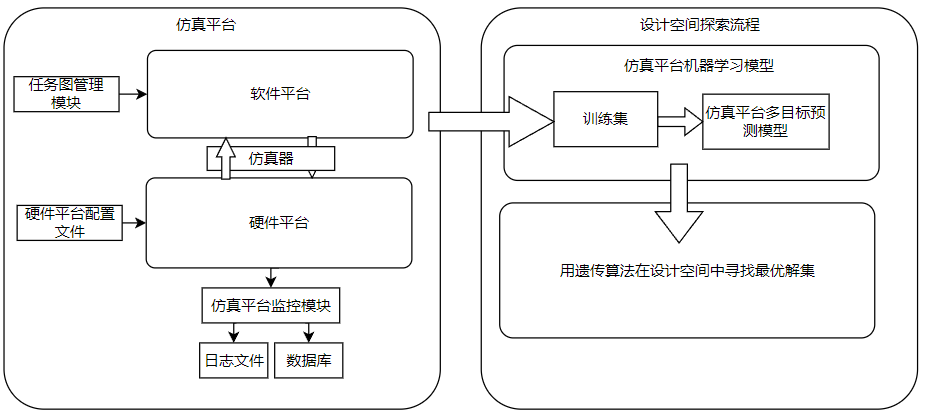
\includegraphics[width=1\textwidth]{系统整体框架图.png}
    \caption{系统整体框架图}
    \label{fig:badge}
\end{figure}

如系统整体框架图可以看出,该系统是一个以仿真平台为基础,实现
通过遗传算法对比较大的设计空间进行探索。我们初期实现TopLevel
仿真平台,仿真平台通过读取硬件配置表实例化硬件平台。随后平台
读取输入的任务图,软件平台读取任务,然后通过调度分到各个硬件
上执行任务,输出日志文件和数据库文件。

通过在仿真平台上快速进行仿真,得出相对于设计空间较小的训练集
文件。训练集文件中包括硬件平台配置,如总线位宽、一个组中DSP
数量、内存大小等等。还包括仿真输出的数据库中提取的仿真信息
,如仿真时延、核利用率、核一致性等等。

然后基于生成的训练集文件,通过现有的机器学习Adaboost模型\cite{29}对
训练集文件训练出仿真平台多目标预测模型\cite{30},最后我们运用遗传算
法对设计空间进行迭代剪枝,最后得出最优的设计种群。

系统主要包括仿真平台和设计空间探索流程两个部分,所以下面就
这两个方面以及仿真结果数据库部分来分别来简要介绍各自的设计。

\section{仿真平台硬件模型生成模块概要设计}
TopLevel仿真平台主要实现硬件平台各个模块的实例化,任务图的
读取以及执行。整个仿真平台模块主要分为ALA调度器模块、Memory
模块、总线模块、处理器模块、用于各模块之间数据以及消息传输的
GeneralFifo模块。仿真平台的整体架构图如图4.2所示:

\begin{figure}[h]
    \centering
    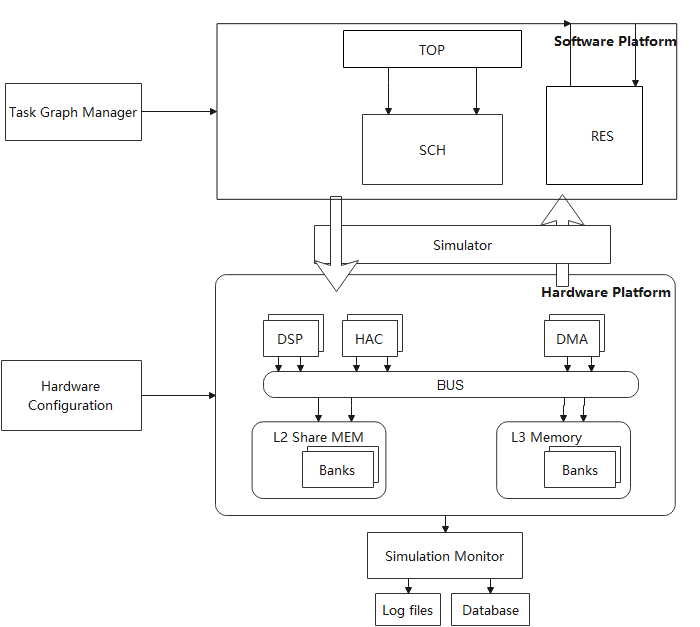
\includegraphics[width=1\textwidth]{仿真平台整体架构图.png}
    \caption{仿真平台整体架构图}
    \label{fig:badge}
\end{figure}

下文主要对仿真平台中设计实现的的硬件平台构建模块、硬件模型生成模块
(Processor模块和Memory模块)以及GeneralFifo模块设计进行简要的介绍。

\subsection{硬件平台构建模块概要设计}
平台开发人员根据仿真平台用户的需求进行建模,提供在系统仿真过程中所需要的各种硬件
模型,用户根据需求构建系统仿真所需的硬件平台。在构建硬件平台时,用户通过修改硬件
平台配置文件中的硬件模块实例信息以及各个实例之间的连接方式,包括每个硬件模块的配
置信息和总线的路由映射。硬件平台的构建过程由下图4.3所示:

\begin{figure}[h]
    \centering
    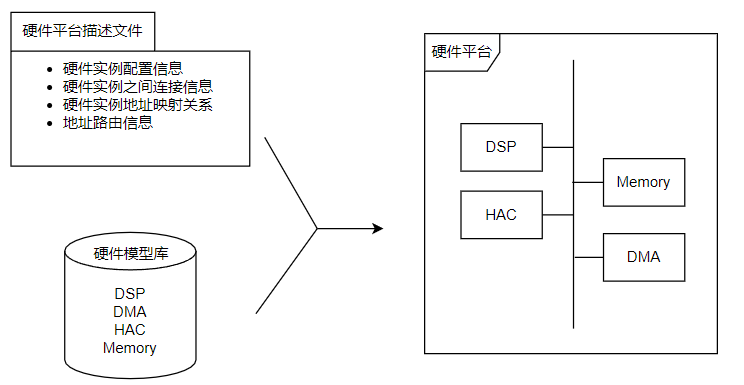
\includegraphics[width=0.8\textwidth]{硬件平台生成图.png}
    \caption{硬件平台生成图}
    \label{fig:badge}
\end{figure}

在仿真平台中,整个硬件系统的构成是一个树状结构的层次化架构,在硬件平台的构建
过程是对该树状结构进行深度优先遍历,所有硬件模型都基于GeneralModule基类实例化。
在硬件平台构建过程中会根据硬件平台配置文件中的配置信息,先实例化最下端叶节点的
各个具体的硬件模型,再去构建上层的分区组件直至整个硬件平台实例化完成。硬件平台
构建的活动图如图4.4所示:

\begin{figure}[h]
    \centering
    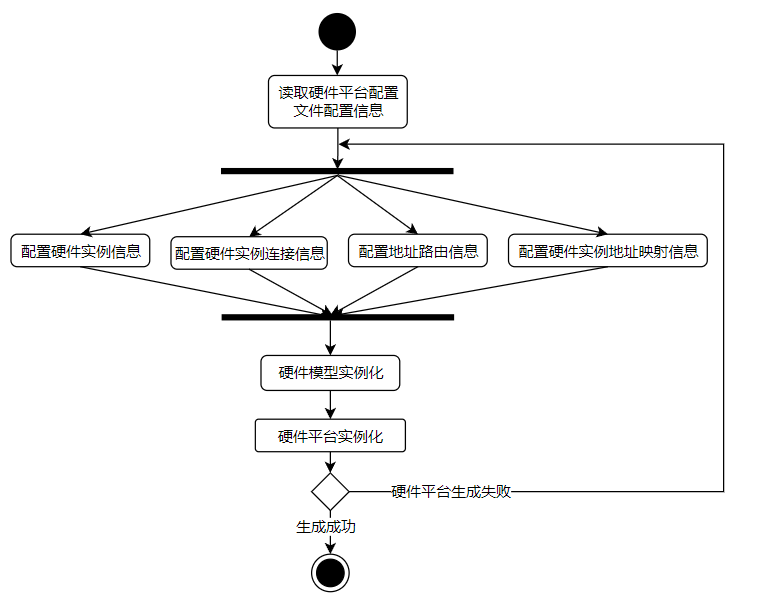
\includegraphics[width=0.9\textwidth]{硬件平台生成活动图.png}
    \caption{硬件平台生成活动图}
    \label{fig:badge}
\end{figure}

如图4.4所示硬件平台在构建过程中,平台需要从硬件模型库中实例化具体的硬件模型
。平台开发人员需要对各种硬件模型进行建模,包括DSP模型、DMA模型以及Memory模型
等等。在构建过程中,系统通过硬件平台配置文件中的硬件模型配置信息去修改硬件模型
库中的硬件模型基类中的可配置参数去实例化具体的仿真平台所需要的硬件模型。在将
建模好的硬件模型基类增加到硬件模型库中之前,通过对硬件模型的单点测试去修改和完善
在设计阶段没有考虑完善的功能需求。同时由于在不同的业务背景下,仿真平台需要不同的硬件
模型,但整体模型基础功能大致相同,所以我们在后续开发其他硬件模型时,只需基于现有
的硬件模型基类去开发,而不需要从零再进行开发。硬件模型库中涉及到多种硬件模型,其中
包括处理器硬件模型、调度器模型、存储器模型以及互联互通模型等。其中处理器模型、存储器
模型的概要设计将在后续几个小节中介绍。

\subsection{GeneralFifo模块概要设计}
GeneralFifo是为了满足模型处理流程需求而开发的一种通用先入先出队列(First in first out,Fifo)
机制\cite{31},可以实现/建模过程中各种前后级同步,反压等需求。它主要有以下几个方面的功能:

\begin{enumerate}
    \item 对连续的数据流进行缓存,防止在存储操作的时候发生数据丢失;
    \item 数据集中起来进行进栈和存储,可避免频繁的总线操作,减轻CPU的负担;
    \item 允许系统进行DMA操作,提高数据的传输速度。
    \item 作为消息队列,支撑仿真平台各个模块之间消息交互,提供事件触发机制。
\end{enumerate}

在硬件设计中,Fifo一般设计为“乒乓”存储方式,在硬件仿真设计中,我们采用以先入先出队列为
存储数据的存储器,GeneralFifo还集成了SimPy里的event机制,实现仿真平台中模块与模块之间的消息交互需求。

GeneralFifo模块通过在模块实例化的时候创建向空队列写对象事件以及从满队列中取
对象事件,当相对应操作出现时,便通过SimPy中的event机制去触发相对应的事件。而
等待该操作的外部模块就可以即时接收到讯息,并即刻执行相对应的操作。这样就实现了
各个模块之间通过GeneralFifo通讯时,当没有对象,进程可以一直等待其他模块传对
象的情形。与此同时,为了实现整个GeneralFifo的事件触发机制,GeneralFifo需要提供队列是
否为空或为满、获取队列的深度以及队列中对象的数量、获取向空
队列写对象事件和从满队列中取对象事件等方法和函数接口。GeneralFifo模块实现流程如图4.5所示:
\\
\\
\\

\begin{figure}[h]
    \centering
    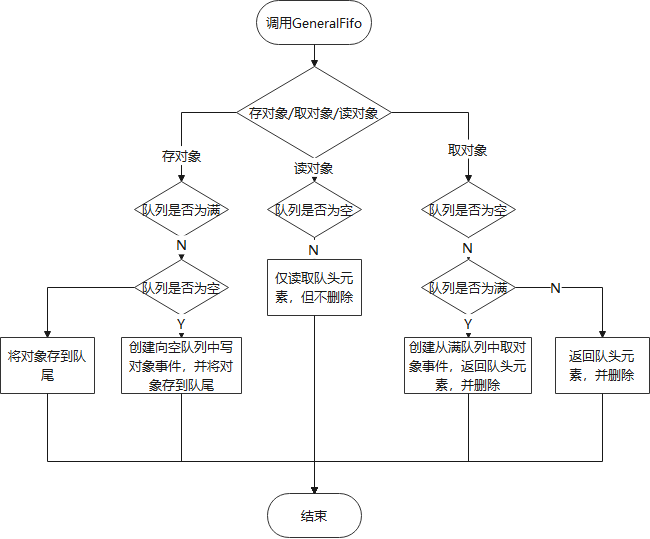
\includegraphics[width=1\textwidth]{GeneralFIFO流程图.png}
    \caption{GeneralFifo流程图}
    \label{fig:badge}
\end{figure}

\subsection{Memory模块概要设计}
Memory模块\cite{32}在整个硬件平台中包括SL2(外部的公共内存池)和PL2
(在每个processor模块内部的内存池)两种内存块。Memory模块根据平台配置
的Bank位宽在模型内部将Memory分为不同的Bank模块,具体的数据读写由内部
Bank模块进行执行。

Processor模块对数据的处理需要从SL2内存池中将数据取到自己内部的PL2内存池中,
再将处理后的数据存到外部的SL2内存池中。Memory模块负责数据的存取处理。Memory
模块接收从总线上传来的读写请求Flit,并根据
位宽将Flit拆分为相应的Bank操作,并将操作处理符发送到到对应Bank
上的Fifo中。Bank模块在硬件平台构建时进行初始化,同时Bank模块创
建bank读写操作进程,一旦有bank读写操作符发送到对应的Fifo中时,
就会触发从Fifo中取出bank读写操作对象,完成开辟bank读写操作符上
所带的读写操作信息,开辟对应地址的内存空间并存储数据或将对应地址
的数据取出并释放该地址的内存空间,并向Memory上的SlavePort
发送读写响应。Memory模块的结构图如图4.6所示:
\\

\begin{figure}[h]
    \centering
    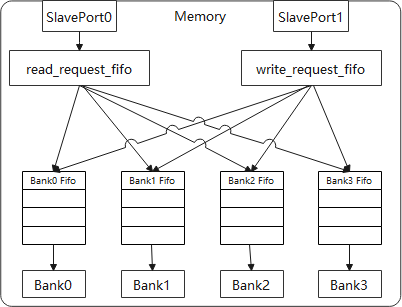
\includegraphics[width=0.8\textwidth]{Memory模块结构图.png}
    \caption{Memory模块结构图}
    \label{fig:badge}
\end{figure}

读写请求通过总线发送到对应Memory模块的SlavePort口,根据请求类型不同
分别发到读请求Fifo上或写请求Fifo上,再根据Bank位宽拆分,发送
到不同Bank上的Fifo中排队,最后由相对应的Bank进行读写请求操作。

\subsection{Processor模块概要设计}
Processor模块对DSP、HAC和DMA三种模型进行建模,实现模型的硬件行为、
建立模型内的流水线结构并实现与其他模块的交互行为\cite{33}。Processor模块现在包括
ProcessorMgnt、ProcessorBase以及具体的DMA、DSP、HAC模型
模块。Processor模块整体结构如图4.7所示:
\begin{figure}[htb]
    \centering
    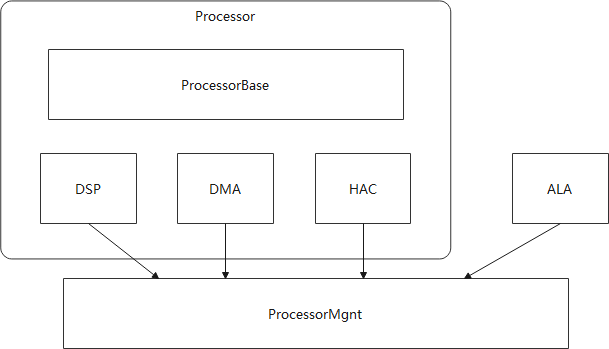
\includegraphics[width=0.8\textwidth]{Processor模块结构图.png}
    \caption{Processor模块结构图}
    \label{fig:badge}
\end{figure}

ProcessorMgnt模块是实现具体模型的管理功能。各个模型(ALA、DSP、
DMA等等)在实例化的时候,ProcessorMgnt记录下对应的对象,并提供
方法给各个模块之间通过内部的Fifo之间交互。这样我们在具体模块之间
进行消息交互的时候不用将消息封装成数据通过总线交互,节省了仿真时
的资源浪费。由于各个模块之间消息交互十分频繁,所以这样也大大提高
仿真平台的仿真效率。

ProcessorBase模块是DMA、DSP及HAC模块的基类,实现了具体模型的基
础功能,并提供相应的接口。ProcessorBase模块实现了模块消息交互以及
添加消息交互接口的功能。

DMA(direct Memory Access, 直接存储器访问)模块负责将数据从一块地
址复制到另一块地址空间,提供在存储器和存储器之间的高速数据传输,在
设计的仿真平台中主要负责PL2内存池和SL2内存池之间的数据传输。

DSP(Digital Signal Processing,数字信号处理)芯片是一种快速强大的微处理器,可以迅速的实现各种数字信号处理算法。
在仿真过程中,DSP模块负责快速完成数据的计算处理。在轻量级仿真平台中,该模块只有数据处理的
时延,不负责数据搬运。只需要体现系统时延,不需要对搬运的数据进行真实的操作。

HAC(Hardware Accelerator,硬件加速器)是用来专门处理某一类执行次数很多的硬件操作的
的硬件,为了加快这一类的操作,特地设计一种芯片专门处理这种操作。HAC模型负责处理
数据搬入、数据处理以及数据搬出的所有操作。

DMA(direct Memory Access, 直接存储器访问)模块负责将数据从一块地
址复制到另一块地址空间,提供在存储器和存储器之间的高速数据传输,在
设计的仿真平台中主要负责PL2内存池和SL2内存池之间的数据传输。

DSP芯片是一种快速强大的微处理器,可以迅速的实现各种数字信号处理算法。
在仿真过程中,DSP模块负责快速完成数据的计算处理,在该模块只有数据处理的
时延,不负责数据搬运。在DSP模块只需要体现系统时延即可。

\section{设计空间构建模块及仿真预测模型概要设计}
设计空间探索是指根据系统设计所关心的参数而对不需要的参数进行系统
分析和修剪。设计空间探索模块实现在可配置的系统资源构成的设计空间中
寻找目标优秀的设计方案。设计空间探索主要分为构建设计空间和选择优化目标、对
设计空间进行剪枝以及对设计空间探索结果分析三个部分。设计空间构成
由可配置的系统参数以及系统参数的可行范围构成,一般而言,设计空间
的整体范围会比较大。优化目标则是我们对整个系统的优化方向,比如在
本文中的设计空间探索流程中,优化目标为仿真时延、核利用率以及核一
致性几个参数。设计空间探索的流程图如图4.8所示:

\begin{figure}[htb]
    \centering
    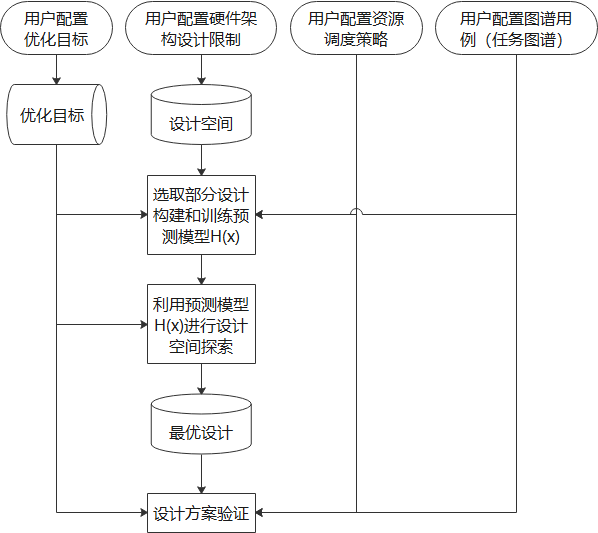
\includegraphics[width=0.9\textwidth]{设计空间探索流程图.png}
    \caption{设计空间探索流程图}
    \label{fig:badge}
\end{figure}

我在设计空间探索模块主要负责的是设计空间的参数提取和构建以及仿真
平台预测模型的设计与实现。

仿真系统中设计空间探索设计流程如图所示,在设计探索流程的具体实现中,
我们先修改仿真平台系统参数,自动化迭
代运行仿真平台,并通过读取数据库信息提取出设计空间探索所有的目标
值,最后将设计方案和对应的仿真数据输出到txt文件中。

将上个流程中提取的6000个训练集数据作为输入数据训练仿真平台预测模
型。最后在遗传算法中探索设计空间中所有设计方案,最后输出最为优秀
的设计种群作为我们设计的备选方案,并对方案重新在仿真平台上运行,
对仿真结果进行对比分析。

下面主要分别设计空间构建模块、探索预测模块的概要设计
进行简要介绍。

\subsection{设计空间构建模块概要设计}
通过对系统设计空间探索的需求分析,找出我们所需要的系统的优化方
向即优化目标,通过分析仿真系统哪几个可配置参数会对优化目标产生较
大影响,提取出这几个设计参数,根据真实芯片设计的参数变化,对设计
参数范围进行限制,最后形成设计空间。
通过对系统设计空间探索的需求分析,我们找出我们需要对系统的优化方
向即优化目标,通过分析仿真系统哪几个可配置参数会对优化目标产生较
大影响,提取出几个设计参数,通过对设计参数范围的限制,最后形成设
计空间。

由于后期在遗传算法进行设计空间探索的过程中进行迭代时,设计空间中
配置参数值的变化要求仿真平台中进行配置参数的调整。

\subsection{仿真平台预测模型概要设计}
设计空间探索流程中遗传算法需要进行多次的仿真过程迭代,为了减少设计
空间探索流程的时间开销,由于在设计空间探索的过程中,仿真平台的配置
参数和目标值固定,所以将系统仿真流程设计成仿真平台预测模型,这样可以大
大减少目标值的输出时间。接下来从训练集生成和预测模型生成两个方面介绍:

训练集生成模块实现的功能包括:读取设计空间中配置并配置到硬件配置
文件中、自动化读取配置文件迭  代运行仿真文件、读取每次仿真结果数据
库文件提取所需要的目标值、将设计方案和对应的目标值输出到文件中并
最终输出训练集文件。该模块的流程图如图4.9所示:

\begin{figure}[htb]
    \centering
    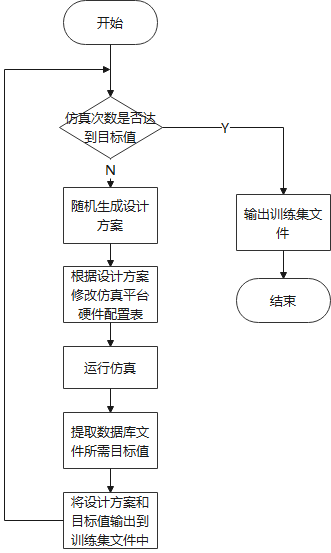
\includegraphics[width=0.5\textwidth]{训练集生成模块流程图.png}
    \caption{训练集生成模块流程图}
    \label{fig:badge}
\end{figure}

训练集文件中的目标值即仿真数据结果,我们需要在每次通过修改硬件配置
在仿真平台上进行系统仿真,在仿真结束后通过对数据库文件中数据的提取
将相应的目标值统计计算到相应的文件中。这样从设计空间中采样得到样本
,将样本在仿真平台上运行得出相应的目标值,从而得到训练集文件。

预测模型生成模块生成仿真平台多目标预测模型,先将上个流程中的数据集经过处理
后提取出来,并分为训练集和验证集。采用现有的sklearn框架中的决策
树回归模型\cite{34}去训练每个目标,再通过一个多目标预测模型类将所有模型
文件读取,并实现预测目标值的功能函数。这样整体每个目标的预测误
差较低。

\section{仿真信息数据库概要设计}
在仿真过程中,我们在每个节点对仿真信息进行统计,最后在仿真结束时
输出至数据库进行整理。从而得到一系列我们对整个仿真过程每个任务的
执行过程,每个硬件的利用率,内存的申请情况,通过这些信息,我们就
可以对整个仿真进行分析,并通过这些输出结果进行下一步DSE架构探索。

仿真系统的结果输出主要通过log信息和数据文件实现,log信息主要统计
任务执行的细节信息,方便寻找调优的关键节点。数据库文件统计任务的
执行过程,每个硬件的利用率,内存的利用等等。仿真平台的数据库采用
python的SQLite库实现。系统中只需在仿真流程中在数据库中各自独立更
新数据库中各个表的数据,每个表的数据表基本独立,SimId是所有数据
表的主键,用于区别多次仿真之间结果。数据库的物理模型由下列各表
所示:

\begin{table}[!h]
    \centering\normalsize
    \caption{SimRecord表}
    \begin{tabular}{|c|c|c|c|c|c|}
    \hline
    \textbf{序号} & \textbf{字段名} & \textbf{字段说明} & \textbf{类型} & \textbf{是否为空} & \textbf{说明} \\ \hline
    1           & SimId        & 仿真序号          & int         & N             &             \\ \hline
    2           & StartTime    & 仿真开始时间        & int         & N             &             \\ \hline
    3           & EndTime      & 仿真结束时时间       & int         & N             &             \\ \hline
    4           & SimTime      & 仿真持续时间        & int         & N             &             \\ \hline
    5           & TestCaseName & 仿真用例名字        & Text        & N             &             \\ \hline
    \multicolumn{2}{|c|}{补充说明} &               &             &               &             \\ \hline
    \end{tabular}
    \note{注:一个数据库可以记录多次仿真的结果,以SimId作为区别。}
    \end{table}

\begin{table}[!h]
    \centering\normalsize
    \caption{AlaKernelTaskTbl表}
    \begin{tabular}{|c|c|c|c|c|c|}
    \hline
    \textbf{序号} & \textbf{字段名} & \textbf{字段说明} & \textbf{类型} & \textbf{是否为空} & \textbf{说明} \\ \hline
    1           & SimId        & 仿真序号          & int         & N             &             \\ \hline
    2           & KernelId     & Kernel任务序号    & int         & N             &             \\ \hline
    3           & InstId       & 任务具体实例序号      & int         & N             &             \\ \hline
    4           & KernelType   & 任务类型          & int         & N             &             \\ \hline
    5           & ReadyTime    & 任务的就绪时间       & int         & N             &             \\ \hline
    6           & IssueTime    & 任务开始执行时间      & int         & N             &             \\ \hline
    7           & CompleteTime & 任务结束执行时间      & int         & N             &             \\ \hline
    8           & PreMoveEnd   & 任务前搬移结束时间     & int         & N             &             \\ \hline
    9           & PostMoveEnd  & 任务后搬移结束时间     & int         & N             &             \\ \hline
    \multicolumn{2}{|c|}{补充说明} &               &             &               &             \\ \hline
    \end{tabular}
    \note{注:AlaKernelTaskTbl表记录的是在Dsp核执行的任务,前搬移任务和后搬移任务分别用来搬运任务的输入数据和输出数据。}
    \end{table}

\begin{table}[!h]
    \centering\normalsize
    \caption{HacJobTable表}
    \begin{tabular}{|c|c|c|c|c|c|}
    \hline
    \textbf{序号} & \textbf{字段名} & \textbf{字段说明} & \textbf{类型} & \textbf{是否为空} & \textbf{说明} \\ \hline
    1           & SimId        & 仿真序号          & int         & N             &             \\ \hline
    2           & JobTypeId    & 任务的序号         & int         & N             &             \\ \hline
    3           & InstId       & 任务具体实例序号      & int         & N             &             \\ \hline
    4           & PipeLine     & 任务具体哪一级流水     & int         & N             &             \\ \hline
    5           & StartTime    & 任务开始执行时间      & int         & N             &             \\ \hline
    6           & EndTime      & 任务结束执行时间      & int         & N             &             \\ \hline
    \multicolumn{2}{|c|}{补充说明} &               &             &               &             \\ \hline
    \end{tabular}
    \note{注:该表记录了Hac任务所处的流水级别和Hac任务在该级流水的执行细节。}
    \end{table}

\begin{table}[!h]
    \centering\normalsize
    \caption{WFEJobTable表}
    \begin{tabular}{|c|c|c|c|c|c|}
    \hline
    \textbf{序号} & \textbf{字段名} & \textbf{字段说明} & \textbf{类型} & \textbf{是否为空} & \textbf{说明} \\ \hline
    1           & SimId        & 仿真序号          & int         & N             &             \\ \hline
    2           & JobTypeId    & 任务的序号         & int         & N             &             \\ \hline
    3           & InstId       & 任务具体实例序号      & int         & N             &             \\ \hline
    4           & StartTime    & 任务开始执行时间      & int         & N             &             \\ \hline
    5           & CompleteTime & 任务结束执行时间      & int         & N             &             \\ \hline
    \multicolumn{2}{|c|}{补充说明} &               &             &               &             \\ \hline
    \end{tabular}
    \note{WFE任务不在核上执行,只起任务的收齐作用,当所准备的任务全部做完后,立刻执行完毕。}
    \end{table}

\begin{table}[!h]
    \centering\normalsize
    \caption{Pl2UsageRecord表}
    \begin{tabular}{|c|c|c|c|c|c|}
    \hline
    \textbf{序号} & \textbf{字段名} & \textbf{字段说明} & \textbf{类型} & \textbf{是否为空} & \textbf{说明} \\ \hline
    1           & SimId        & 仿真序号          & int         & N             &             \\ \hline
    2           & TTI          & 仿真时间段         & int         & N             &             \\ \hline
    3           & SimTime      & 记录的时间点        & int         & N             &             \\ \hline
    4           & AlaId        & 调度器Id         & int         & N             &             \\ \hline
    5           & PoolId       & 内存池Id         & int         & N             &             \\ \hline
    6           & UsedSize     & 内存池已使用的大小     & int         & N             &             \\ \hline
    7           & AllocSize    & 内存池已分配的大小     & int         & N             &             \\ \hline
    \multicolumn{2}{|c|}{补充说明} &               &             &               &             \\ \hline
    \end{tabular}
    \note{注:该表记录了Pl2内存的在每个时间段的使用情况,以内存池为单位进行记录。}
    \end{table}

\begin{table}[!h]
    \centering\normalsize
    \caption{SimUsageTable表}
    \begin{tabular}{|c|c|c|c|c|c|}
    \hline
    \textbf{序号} & \textbf{字段名}  & \textbf{字段说明} & \textbf{类型} & \textbf{是否为空} & \textbf{说明} \\ \hline
    1           & SimId         & 仿真序号          & int         & N             &             \\ \hline
    2           & ProcessorName & 硬件名称          & text        & N             &             \\ \hline
    3           & TTI           & 仿真时间段         & int         & N             &             \\ \hline
    4           & SampleCount   & 时间片序号         & int         & N             &             \\ \hline
    5           & Usage         & 时间片内硬件利用率     & int         & N             &             \\ \hline
    \multicolumn{2}{|c|}{补充说明} &               &             &               &             \\ \hline
    \end{tabular}
    \note{注:该表记录了在仿真过程中每个时间片内硬件资源的利用率。}
    \end{table}

\begin{table}[!h]
    \centering\normalsize
    \caption{DBMUsageRecord表}
    \begin{tabular}{|c|c|c|c|c|c|}
    \hline
    \textbf{序号} & \textbf{字段名} & \textbf{字段说明} & \textbf{类型} & \textbf{是否为空} & \textbf{说明} \\ \hline
    1           & SimId        & 仿真序号          & int         & N             &             \\ \hline
    2           & TTI          & 仿真时间段         & int         & N             &             \\ \hline
    3           & SimTime      & 记录的时间点        & int         & N             &             \\ \hline
    4           & AlaId        & 调度器Id         & int         & N             &             \\ \hline
    5           & PoolId       & 内存池Id         & int         & N             &             \\ \hline
    6           & UsedSize     & 内存池已使用的大小     & int         & N             &             \\ \hline
    7           & AllocSize    & 内存池已分配的大小     & int         & N             &             \\ \hline
    \multicolumn{2}{|c|}{补充说明} &               &             &               &             \\ \hline
    \end{tabular}
    \note{注:该表记录了仿真过程中以DBM管理的Sl2内存每个时间段的分配情况,以内存池为单位记录。}
    \end{table}

~\\
\section{本章小结}
本章基于仿真平台的的整体设计及设计空间探索的整体框架入手,详细介绍
了仿真平台的整体流程以及相关模块的架构以及功能实现、设计空间探索模
块的主要流程以及各个流程模块里面的功能实现,如何生成训练集以及预测
模型的训练生成等等。

本章为系统的详细设计提供了明确的框架,表明了设计开发的重点和难点,
为后续系统的具体设计提供了有力的帮助。